%
% $RCSfile: common_and_crosscutting_concerns.tex,v $
%
% Copyright (C) 2002-2008. Christian Heller.
%
% Permission is granted to copy, distribute and/or modify this document
% under the terms of the GNU Free Documentation License, Version 1.1 or
% any later version published by the Free Software Foundation; with no
% Invariant Sections, with no Front-Cover Texts and with no Back-Cover
% Texts. A copy of the license is included in the section entitled
% "GNU Free Documentation License".
%
% http://www.cybop.net
% - Cybernetics Oriented Programming -
%
% http://www.resmedicinae.org
% - Information in Medicine -
%
% Version: $Revision: 1.1 $ $Date: 2008-08-19 20:41:05 $ $Author: christian $
% Authors: Christian Heller <christian.heller@tuxtax.de>
%

\subsection{Common- and Crosscutting Concerns}
\label{common_and_crosscutting_concerns_heading}
\index{Aspect Oriented Programming}
\index{AOP}
\index{Object Oriented Programming}
\index{OOP}
\index{Common Concern}
\index{Crosscutting Concern}
\index{Development Concern}
\index{Production Concern}
\index{Classification of Concerns}

Section \ref{aspect_oriented_programming_heading} argumented that, after
\cite{aspectj}, \emph{Aspect Oriented Programming} (AOP) were necessary because
some concerns were not easily turned into \emph{Classes} -- the natural unit of
modularity for \emph{Object Oriented Programming} (OOP) -- because they'd cut
across classes. Much like OOP were a way of modularising \emph{Common Concerns},
AOP were a way of modularising \emph{Crosscutting Concerns}. Figure
\ref{concerns_figure} is a trial to classify both kinds. (The distinction into
\emph{Development-} and \emph{Production Concerns} is of minor importance here.)

\begin{figure}[ht]
    \begin{center}
        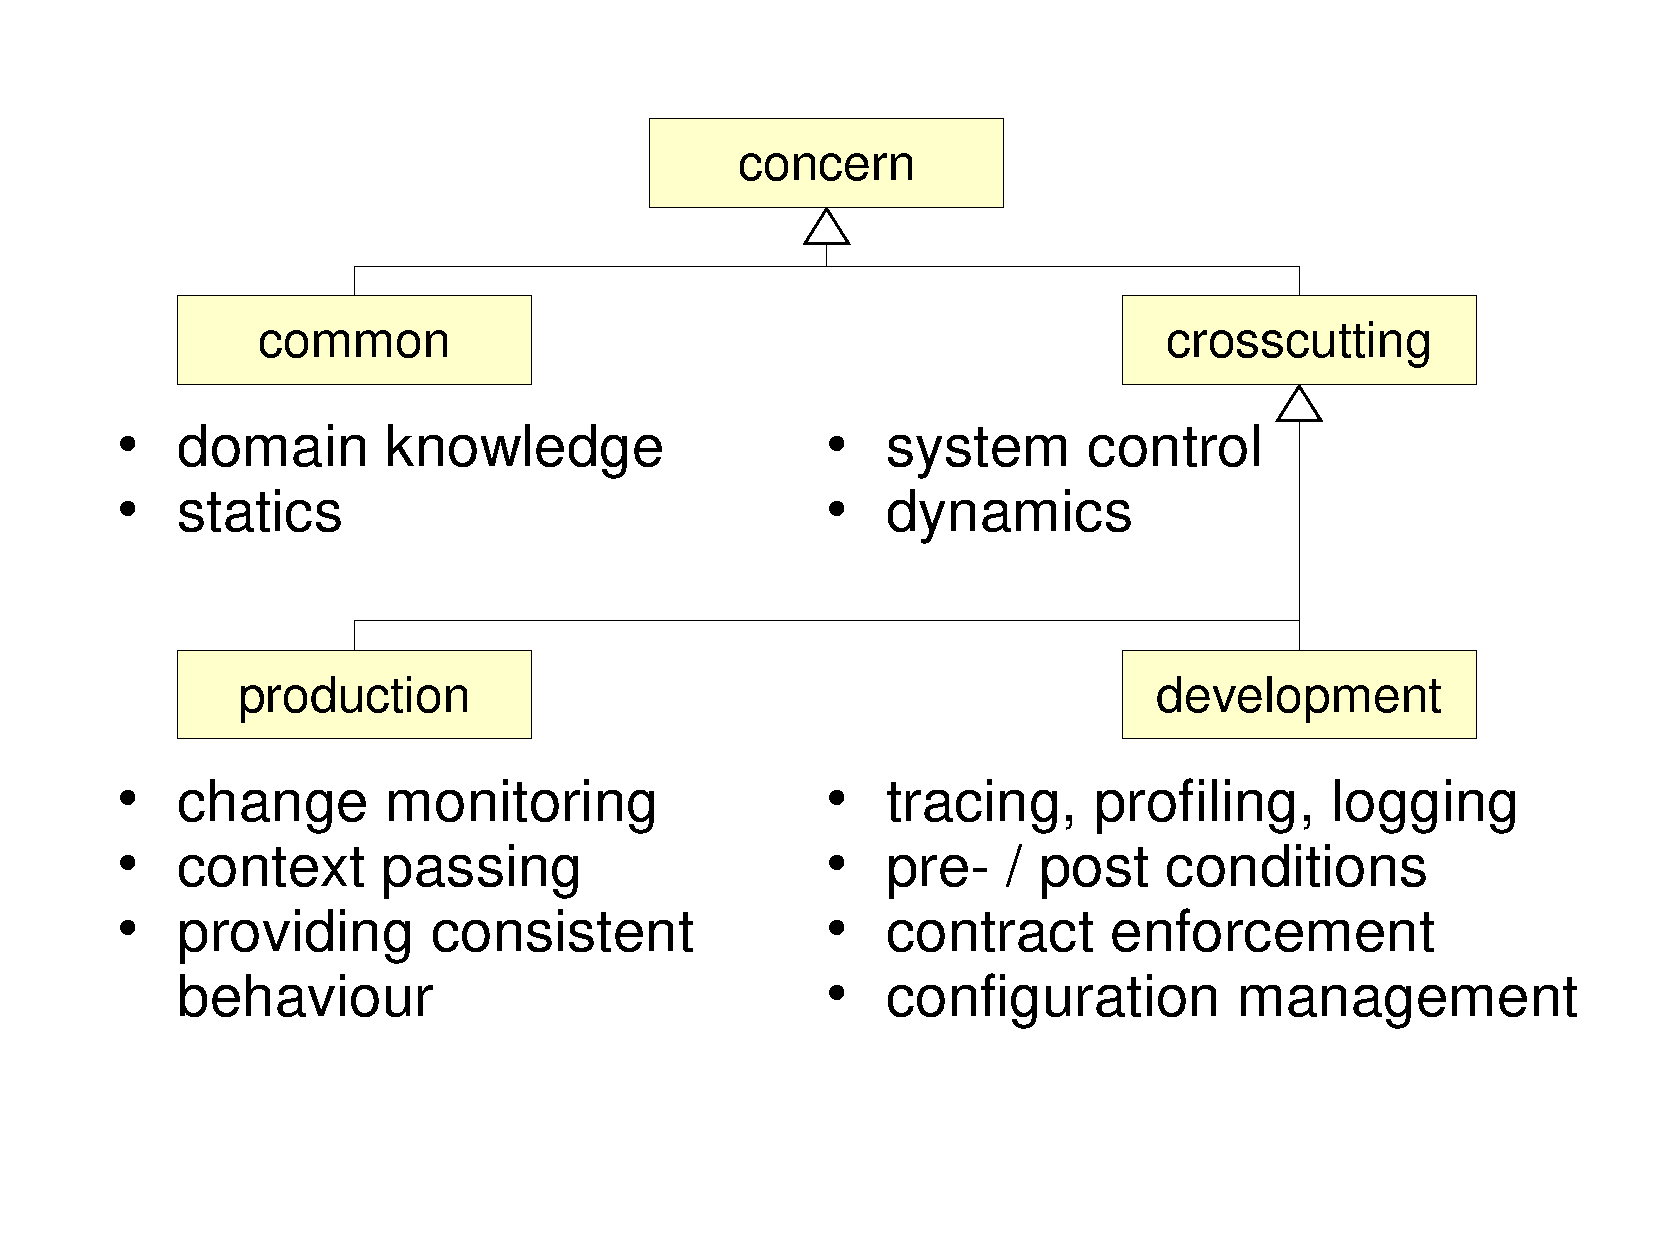
\includegraphics[scale=0.3,angle=-90]{graphic/concerns.pdf}
        \caption{Classification of Concerns}
        \label{concerns_figure}
    \end{center}
\end{figure}

Looking closer at these, it becomes obvious that crosscutting concerns represent
general \emph{System Control} functionality, while common concerns stand for
properties specific to an \emph{Application}. Comparing with nature (section
\ref{virtual_and_real_world_heading}), the separation of both kinds of concerns
seems absolutely correct. It arises the question, however, if AOP with all its
additional concepts is really the most suitable way for treating crosscutting
concerns? This work means \emph{no} and suggests to simply put all general
control functionality into a basic knowledge-interpreter system underlying all
applications (chapter \ref{cybernetics_oriented_interpreter_heading}).
